\section{Dense Object Nets}

\ac{DON} is a recently proposed self-supervised contrastive \ac{DNN} framework.
The framework's network architecture is based on adaptation of SimCLR\cite{simclr} architecture.
While the SimCLR architecture encodes the entire image to an embedding of dimension using
the contrastive loss function as described in Equation~\ref{eqn:simclr}, the \ac{DON}, encodes each pixel in an image to embedding space called dense object descriptors as described in Equation~\ref{eqn:don}.
The image with dense object descriptors as pixels is referred as dense descriptor image.

\begin{figure}[htb]
    \centering
    \caption{\ac{DON} architecture.}
    \label{fig:don_architecture}
    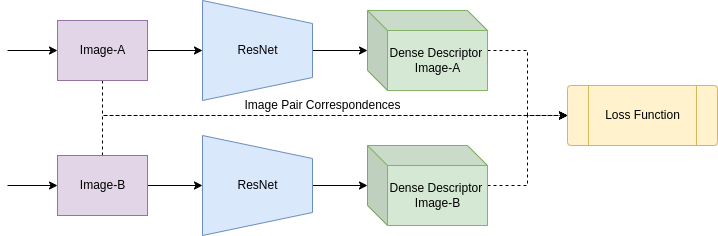
\includegraphics[scale=0.4]{images/don/don_architecture.png}
\end{figure}

\begin{equation}
    \label{eqn:simclr}
    f_{SimCLR}:I \in \mathbb{R}^{H \times W \times 3} \rightarrow x \in \mathbb{R}^D \quad ,\acs{s.t.} \ D \in \mathbb{N}^+.
\end{equation}

\begin{equation}
    \label{eqn:don}
    f_{DON}:I \in \mathbb{R}^{H \times W \times 3} \rightarrow I_D \in \mathbb{R}^{H \times W \times D} \quad ,\acs{s.t.} \ D \in \mathbb{N}^+.
\end{equation}

Furthermore, according to \citeauthor{adrian2022efficient}~\cite{adrian2022efficient}, \ac{DON} relies on sequence of images in the dataset to embed each pixel
to descriptor space by exploiting the geometric prior of objects based on color-hues inturn, generalizing the object.\\

The \ac{ResNet} is usually optimized using mutual image correspondence information of image pairs with contrastive learning on a pixel scale.
The trained network computes a embeddings \ac{s.t.}
the pixel has an unique embedding compared to the rest of the pixels.
The network's visual embedding is invariant to a viewpoint and illumination and comes with the inherent property of generalizing same-class objects.
The visual embedding uniquely describes the pixel locally in an image; hence, referred to as a local descriptor.
The contribution of \ac{DON} is thus its immense ability to generalize for other similar objects within a class without a need to train the network for each such object.



\subsection{Implementation Strategy}

Introduced in 2019, \ac{DON} is young in the research field and applied for use cases in 2021.
In earlier years, the authors of \ac{DON} proposed ``Pixelwise Distribution Loss'' to improve ``Pixelwise Contrastive loss''. This year,
researchers \citeauthor{adrian2022efficient}~\cite{adrian2022efficient} introduced a new loss function called ``Pixelwise NT-Xent Loss'' to make \ac{DON} robust.
The implemented use cases \parencites{rope-manipulation}{block-manipulation}{florence2019self} used different \ac{ResNet} architecture variants
giving an opportunity to test combinations of loss functions with architectures to optimize the network.



\subsection{ResNet Architectures}
\ac{ResNet}-$N$ means that the \ac{DNN} has $N$ convolution layers with shortcuts between them aiding better optimization \cite{resnet}.
E.g., \ac{ResNet}-34 consists of 34 weighted layers. Originally proposed, \ac{ResNet}-34 came with few design rules; to maintain the temporal complexity per layer, the layers had the same number of
filters for the same output feature map size, and the number of filters doubled in that scenario.
The identity shortcuts were employed directly as the input and output dimensions stand the same.\\

With an increase in dimensions, there were two options to consider.
The initial assumption was that the shortcut would continue to conduct identity mapping while padding extra zero entries for expanding dimensions.
The other option was to utilize the projection shortcut to match dimensions.\\

The \ac{ResNet}-50 inherits architecture from the \ac{ResNet}-34 model, with revision in the bottleneck design.
Each of the \ac{ResNet}-34's 2-layer blocks was replaced with a 3-layer bottleneck block, resulting in the deeper \ac{ResNet}-50 design.



\subsection{Loss Functions}


\subsubsection{Pixelwise Contrastive Loss}

The pixelwise constrastive loss is adapted from \cite{simclr} on a pixelwise scale.
The pixelwise contrastive loss brought in the concept of \ac{DON} itself introduced by \citeauthor{florence2018dense}~\cite{florence2018dense}.
The pixelwise constrastive loss function aims
to minimize the distance between the embeddings corresponding to a match, while the embeddings corresponding to
a non-match are set at least by a marginal distance $M$ apart. The loss function is described as,

\begin{equation}
    \mathcal{L}_{matches} = \dfrac{1}{N_{matches}} \displaystyle\sum^{N}_{i, j} \left\Vert f(I_a)[x_i, y_j] - f(I_b)[x_i, y_j] \right\Vert,
\end{equation}

\begin{equation}
    \mathcal{L}_{non-matches} = \dfrac{1}{N_{non-matches}} \displaystyle\sum^{N}_{i, j} max(0, \ M - \left\Vert f(I_a)[x_i, y_j] - f(I_b)[x_i, y_j] \right\Vert),
\end{equation}

\begin{equation}
    \mathcal{L}_{Total} = \mathcal{L}_{matches} + \mathcal{L}_{non-matches}.
\end{equation}

$M$ is a hyperparameter and has to be chosen optimally while training the network.
The loss function is sensitive to batch size and number of correspondences \parencites{adrian2022efficient}{florence2020dense}.
Additionally, non-matching correspondences needs to be sampled for training the network.
This thesis is not going to benchmark this loss function as it is outdated and comes with drawbacks compared to newly proposed loss functions.


\subsubsection{Pixelwise Distribution Loss}

Introduced in \citeauthor{florence2018dense}~\cite{florence2018dense}, the pixelwise distribution loss function aims to compute a set of probability distributions for each keypoint $k = \{1, 2, \ldots K\}$
minimizing the divergence between the predicted heatmap and the ground truth heatmap described as,

\begin{equation}
    \label{eqn:spat_exp}
    p_a(x_i, y_i | f(I_a), f(I_b), x_b, y_b) = \dfrac{K(f(I_b)[x_b, y_b], f(I_a)[x_i, y_j])}{\displaystyle\sum_{i', j'}K(f(I_b)[x_b, y_b], f(I_a)[x_i', y_j'])},
\end{equation}

\noindent where, the $K:(\mathbb{R}^{\mathbb{N}^+}, \mathbb{R}^{\mathbb{N}^+}) \rightarrow \mathbb{R}$ is a kernel function and
it can be of any formulation as long as it yields a scalar ($\mathbb{R}$) processing two vectors of the same dimension.
The term, $p_a(x_i, y_i | f(I_a), f(I_b), x_b, y_b) \in [0, 1]$ is the spatial probability of a keypoint in $f(I_a)[x_a, y_a]$ in the image $f(I_b)$.\\

The spatial expectation from the spatial probability is computed as,

\begin{equation}
    \label{eqn:x_exp}
    \hat{x_b} = \displaystyle\sum_i^W p_a(x_i | f(I_a), f(I_b), x_b) x_i,
\end{equation}

\begin{equation}
    \label{eqn:y_exp}
    \hat{y_b} = \displaystyle\sum_i^H p_a(y_i| f(I_a), f(I_b), y_b) y_i,
\end{equation}

The spatial loss of $I_a[x_a, y_a]$ in $I_b[x_b, y_b]$ is computed as,

\begin{equation}
    \mathcal{L}_{b \rightarrow a} = \| x_b - \hat{x_b} \| + \| y_b - \hat{y_b} \|,
\end{equation}

The total bi-directional loss is computed as,
\begin{equation}
    \mathcal{L}_{Total} = \mathcal{L}_{b \rightarrow a} + \mathcal{L}_{a \rightarrow b},
\end{equation}

The kernel functional chosen to compute the bi-directional loss function,
\begin{equation}
    K: (f(I_a)[x_i, y_i], f(I_b)[x_b, y_b]) \rightarrow exp(-\|f(I_a)[x_i, y_i] - f(I_b)[x_b, y_b] \|).
\end{equation}

\begin{figure}[htb]
    \centering
    \captionsource{2D spatial expectation of keypoint in two images.}{\cite{florence2020dense}}
    \label{fig:spat_exp}
    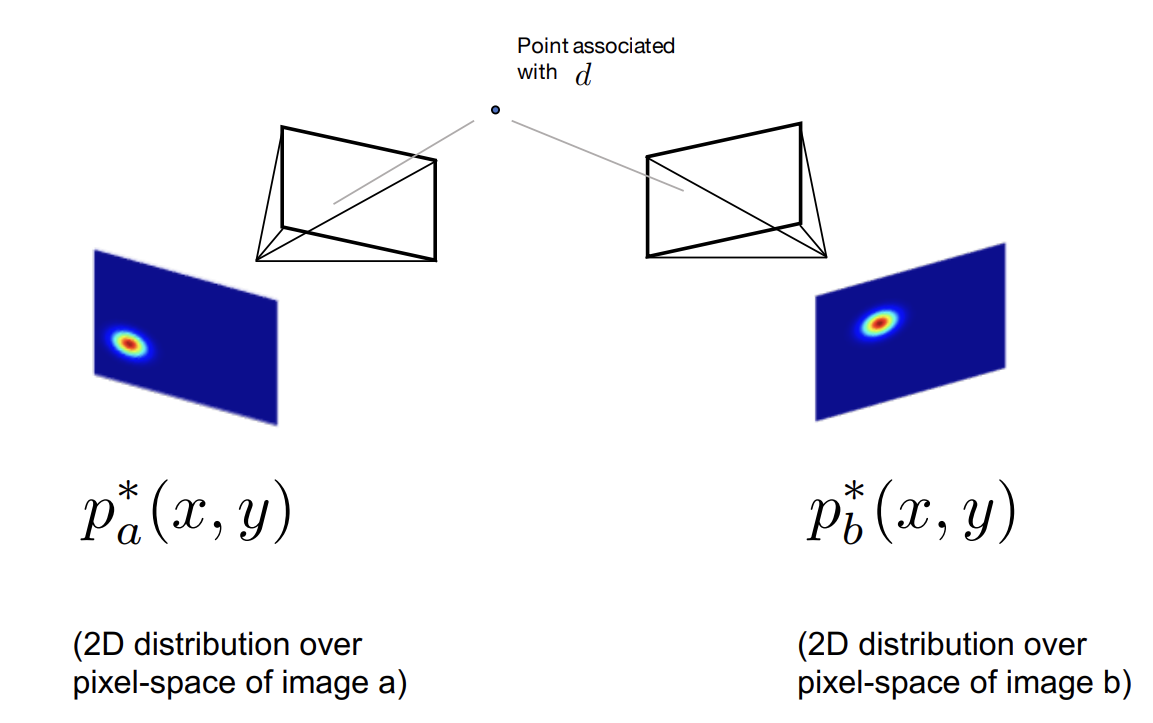
\includegraphics[scale=0.17]{images/spatial_expectation.png}
\end{figure}

This pixelwise distribution loss function can be implemented in a batch fashion yielding high-performance computation time in a computer.
Furthermore, The Figure~\ref{fig:spat_exp} intuitively illustrates the spatial expectation of a keypoint in two images.\\

Furthermore, the loss function improves spatial expectation of a descriptor compared to the pixelwise contrastive loss,
yielding better results in the search space of a descriptor in a new image.
One of the drawbacks of using this loss function is that only one object belonging to the same class in an image can
be used while training the neural network. Having more objects belonging to the same class yields faulty prediction of spatial expectations.

\subsubsection{Pixelwise NT-Xent Loss}

The ``NT-Xent loss'' is originally introduced in \citeauthor{simclr}~\cite{simclr} adopted by \citeauthor{infonce}~\cite{infonce} to encode an entire image to an embedding and implemented on a pixel level
to train \ac{DON} by \citeauthor{adrian2022efficient}~\cite{adrian2022efficient}. The authors \citeauthor{adrian2022efficient}~\cite{adrian2022efficient} randomly sample $N$ correspondences from an
image pair $(I_A, I_B)$, with each correspondence yielding two descriptors $d^A_i$ and $d^B_i$ , for a total of $N$ pairs, or
$2N$ descriptors. For a given descriptor, all other $2(N - 1)$ descriptors are respectively treated as negative examples.
The below given loss function is directly optimized against the descriptor pair,

\begin{equation}
    \mathcal{L}_{i, j} = -\log \dfrac{\exp(K(d_i, d_j) / \tau)}{\sum^{2N}_{k=1, k \neq i} \exp(K(d_i, d_j) / \tau)},
\end{equation}

where, $\tau \in \mathbb{R}^+$ is a temperature scaling factor and $K$ is cosine similarity kernel defined as,

\begin{equation}
    \label{eqn:cosine_similarity}
    K = \dfrac{\left< d_i, d_j \right>}{\| d_i\| \| d_j\|} \quad ,\ac{s.t.} \ d_{i, j} \in \mathbb{R}^{\mathbb{N}^+}, \ K \in  [1, 0].
\end{equation}

Since $K$ takes only positive inputs, unlike the cosine function, it produces the outputs in the range [0, 1] which leads to its interpretation as in expression refer equation \ref{eqn:kernel}.

\begin{equation}
    \label{eqn:kernel}
    K(d_i, d_j) = \begin{cases}
        1 & \implies (d_i, d_j) \text{ are similar}.    \\
        0 & \implies (d_i, d_j) \text{ are dissimilar}.
    \end{cases}
\end{equation}

One of the drawbacks of the pixelwise nt-xent loss function is that semantically closer objects in an image are treated as two different objects which in turn
hinders the generalizing properties of the neural networks.

\subsection{$PCK@k$ as an Evaluation Metric}

To measure the performance of the network, ``$PCK@k$'' evaluation metric is adopted as in preceding works \parencites{pck}{adrian2022efficient}. $PCK@k$ is defined
for a set of pixel pairs $\mathcal{T} = \{p_i, q_i \}^N_{i=1}$ as follows,

\begin{equation}
    \label{eqn:pck}
    PCK@k(\mathcal{T}) = \dfrac{1}{|\mathcal{T}|} \displaystyle\sum_{(p_i, q_i) \in \mathcal{T}} [ \|p_i - q_i\| \leq k] \quad ,\ac{s.t.} \ (p_i, q_i) \in \mathbb{R}^{\mathbb{N}^+}, (k, \mathcal{T}) \in \mathbb{R},
\end{equation}

\noindent where $k$ is the maximum error allowed in turn, influencing the Iverson bracket $[ \ \cdot \ ]$  to 1 if the error is within the limits of $k$ and 0 otherwise.
$\mathcal{T}$ is a number of keypoints ($p_i, q_i$) normalizing the computed metric. Instead of using $L^2$-Norm to compute the error between keypoints, it
is replaced by a kernel function `$D$' similarly in equation~\ref{eqn:cosine_similarity} in page~\pageref{eqn:cosine_similarity} bringing in more flexibility.
The kernel revised metric is described as,

\begin{equation}
    PCK@k(\mathcal{T}) = \dfrac{1}{|\mathcal{T}|} \displaystyle\sum_{(p_i, q_i) \in \mathcal{T}} D(p_i, q_i) \leq k.
\end{equation}


\subsection{Suzanne, a synthetic dataset}

To train and benchmark \ac{DON}, no compatible ready datasets are available. The datasets available either missed camera information like intrinsics or extrinsics parameters,
masks information or captured same objects belonging to the same
class in an image, posing ill-conditions to benchmark pixelwise distribution loss.\\

To overcome this situtation, `BlenderProc'~\cite{blenderproc} is used to generate synthetic dataset with all annotations needed to train \ac{DON}.
`Suzanne' is a model already available in the render tool and is
placed in the world datum center. For this control dataset, 100 random cameras are added in the environment with random poses capturing depth,
extrinsic information and mask for each viewpoint. The Table~\ref{table:suzanne} in page~\pageref{table:suzanne},
provides the preview of dataset. The annotated pixels in blue in second image from right to left in Table~\ref{table:suzanne} projects the correspondences through world
coordinates in the first image from right to left annotated in red. As the dataset produces perfect depth maps of the objects in the images,
the benchmarking metrics might not tally with available benchmarked results.\\


\begin{table}[htb]
    \centering
    \begin{tabular}{ccccc}
        \hline
        \multicolumn{5}{c}{Dataset Preview}                                                                                                                                                                                                                                                                                                                                                               \\ \hline
        \multicolumn{1}{c}{RGB}                                                    & \multicolumn{1}{c}{Depth}                                                 & \multicolumn{1}{c|}{Mask}                                                    & \multicolumn{2}{c}{Correspondences Mapping}                                                                                                               \\
        \multicolumn{1}{c}{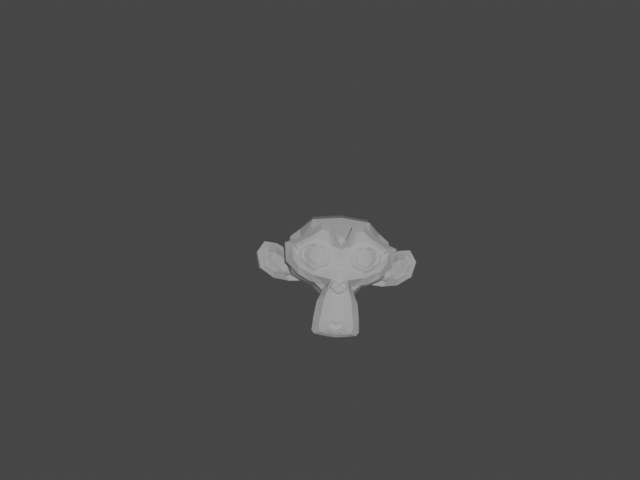
\includegraphics[scale=0.12]{images/suzanne/9_rgb.png}} & \multicolumn{1}{c}{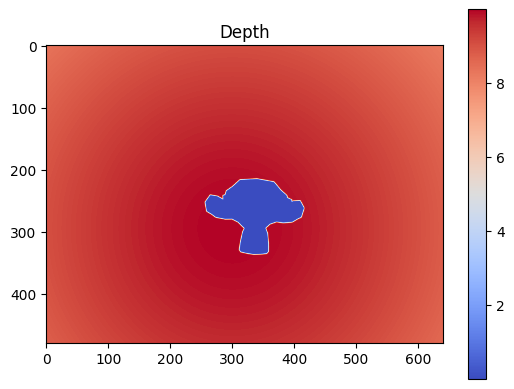
\includegraphics[scale=0.2]{images/suzanne/depth.png}} & \multicolumn{1}{c|}{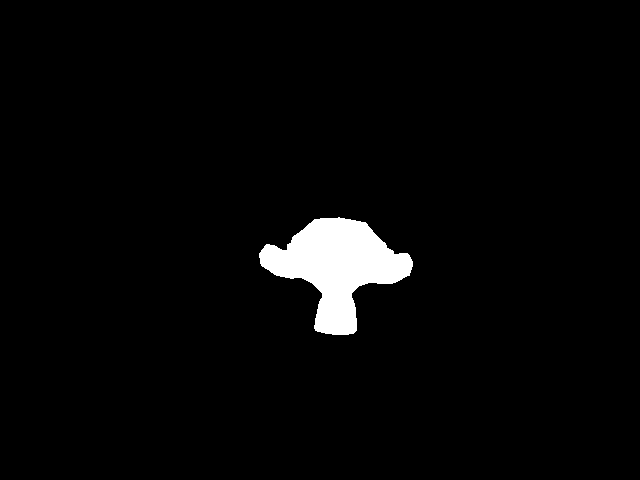
\includegraphics[scale=0.12]{images/suzanne/9_mask.png}} & \multicolumn{1}{c}{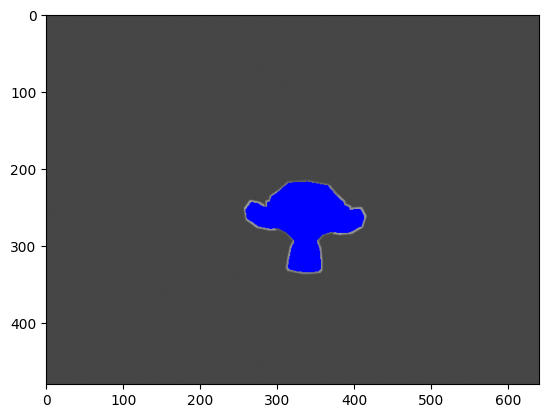
\includegraphics[scale=0.2]{images/suzanne/output.png}} & \multicolumn{1}{c}{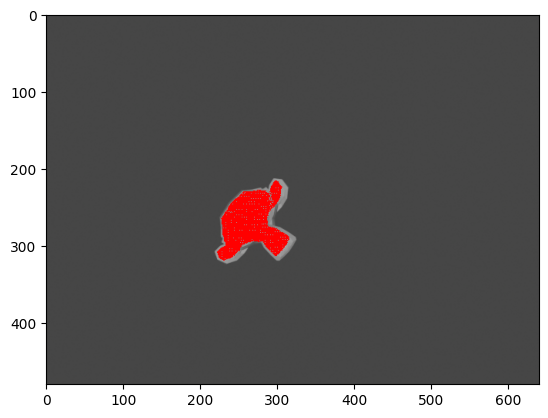
\includegraphics[scale=0.2]{images/suzanne/output_1.png}} \\ \hline
    \end{tabular}
    \caption{Depiction of dataset quintennsials features of dataset}
    \label{table:suzanne}
\end{table}



Following the procedure in \cite{hartley2003multiple}, the correspondences are computed in an image pair described as follows:

\noindent The camera extrinsic parameters ($\mathcal{T}_{C \rightarrow W} \in \mathbb{R}^{4 \times 4}$) is the camera pose relative to the world frame.
The camera intrinsics is defined as $\mathcal{I} \in  \mathbb{R}^{3 \times 3}$.
To map the correspondences from image $I_a$ to image $I_b$, the pixels from the image $[u,v]^T \in I_a \in \mathbb{R}^{2 \times 1}$
are projected to the world coordinates $W_a \in \mathbb{R}^{3 \times 1}$ using depth ($d$) and from the world coordinates to the image $I_b$ as follows:

\begin{equation}
    \label{eqn:world_proj}
    W_a = \mathcal{T}_{C \rightarrow W}^a \ \mathcal{I}^{-a} \ \begin{bmatrix}
        u^a \\
        v^a \\
    \end{bmatrix} \ d_{uv}^a
\end{equation}

The computed world coordinates from $I_a$, $W_a$ are projected to pixels in $I_b$,

\begin{equation}
    d_{uv}^b \ \begin{bmatrix}
        u^b \\
        v^b \\
    \end{bmatrix} =  \mathcal{I}^b \ \mathcal{T}_{C \rightarrow W}^{-b} \ W_a,
\end{equation}

\noindent where,
\begin{equation}
    \mathcal{T}_{C \rightarrow W}^{-b} = \begin{bmatrix}
        R^b   & -R^b t^b \\
        0^T_3 & 1
    \end{bmatrix}, \quad \ac{s.t.} \ R^b \in SO(3).
\end{equation}

Additionally, mask is used to sample the pixels from $I_a$ within the object silhouette.



\subsection{Manual Method for Robot Grasp Generation}

The \ac{DON} produces visual embeddings ($f(I)[u, v] \rightarrow d, \quad d \in \ \mathbb{R}^{\mathbb{N}+}$) such that each pixels withholds unique embedding in descriptor space
reducing computational complexity to find the same pixel in different viewpoint in an \ac{RGB} space omitting complex search algorithm. Using ``Pygame'' \cite{pygame} library in python, an interactive
application is developed to pick descriptors in the descriptor space with it's image coordinates {$[u, v]^T$} using depth and camera intrinsics to project them to the coordinates in the camera frame. More than
three descriptors are picked such that it produces a valid rotation matrix via \ac{PCA} or \ac{SVD} and the mean value acting as a center to generate a 6D pose defined as,

\begin{equation}
    \mathcal{T} = \begin{bmatrix}
        R     & t \\
        0^T_3 & 1
    \end{bmatrix} \in \mathbb{R}^{4 \times 4}, \quad \ac{s.t.} \ R \in SO(3), \ t \in \mathbb{R}^{3 \times 1},
\end{equation}

The interactive application allows to save multiple object pose definition file and this definition file is loaded into an other application to search and compute multiple object
6D pose information in an other or same image. The descriptors are searched using gaussian kernel derived from heat kernel formulation,

\begin{equation}
    \label{eqn:gaussian_kernel}
    \mathbb{E}{[u^*, v^*]_{d}} = \operatorname*{argmin}_{u_i, v_i} \ exp-\left(\dfrac{\|(f(I_a)[u_i, v_i] - d)\|}{exp(t)}\right)^2
\end{equation}

Where $t \in \mathbb{R}$ controls the kernel width influencing the search space to compute the spatial expectation of the query descriptor $d$ in image $I_a$.
The descriptors produced by \ac{DON} are supposedly to be robust against color jitters, illumination changes and occlusions in order to produce consistent 6D poses \cite{adrian2022efficient}.\\

To compute the relative 6D pose of an object in the new viewpoint of the camera, the queried keypoint locations are redordered in the matrix respective to the keypoint
and its spatial locations as stored in the definition file.
If a keypoint is not found, then the keypoint in the definition file is omitted and mutually rearranged. The queried keypoint locations produce relative 6D pose $\mathcal{T}_{object}$
compared to the pose stored in the definition file as,

\begin{equation}
    \mathcal{T}_{rel} = (\mathcal{T}_{def}^T \ \mathcal{T}_{def})^{-1} \ \mathcal{T}_{def}^T \ \mathcal{T}_{object}.
\end{equation}

To eliminate the manual process of annotating keypoints to genetate robot grasps, KeypoinNet is implemented.
